\chapter{Pendahuluan}
\label{chap:intro}

Pada Bab satu akan dibahas pendahuluan dari penelitian yang dilakukan. Bab satu terbagi dalam delapan \textit{sub bab}, yaitu \textit{latar belakang}, \textit{rumusan masalah}, \textit{tujuan}, \textit{batasan masalah}, \textit{ruang lingkup masalah}, \textit{metode penelitian}, \textit{teknik pengumpulan data}, dan \textit{sistematika penulisan}.

\section{Latar Belakang}
\label{sec:latar_belakang}
%Pragraf 1 latar belakang berisi alasan & cerita
\hspace{0.5cm} Transportasi menjadi bagian yang penting bagi manusia di saat penelitian ini dilakukan. Ada dua jenis transportasi bagi seseorang yaitu kendaraan umum dan kendaraan pribadi. Kenyataannya pada saat penelitian ini dilakukan banyak yang lebih memilih kendaraan pribadi dibanding kendaraan umum. Maraknya penggunaan kendaraan pribadi dan penambahan jalur kendaraan yang tidak sebanding banyaknya kendaraan menimbulkan kemacetan. Maraknya penggunaan kendaraan pribadi dikarenakan kurang nyamannya kendaraan umum dan kesulitan dalam menentukan kendaraan umum yang harus dinaiki. Banyaknya rute kendaran umum membuat orang kebingungan dalam memilih kendaraan umum menuju lokasi yang diinginkan. Seseorang cenderung malas untuk bertanya dan mencari rute yang efisien. Karena hal tersebut, seseorang lebih memilih menggunakan kendaraan pribadi ketimbang kendaraan umum. 

%Pragraf 2 latar belakang berisi keinginan pemilihan topik berdasarkan Kiri API
\hspace{0.5cm} Ide pembuatan aplikasi yang memudahkan seseorang dalam menentukan rute kendaraan umum sudah lebih dulu ada yang dikenal dengan nama Kiri. Kiri dibuat dengan latar belakang \\ tiga masalah besar yaitu pemanasan global, kemacetan, dan harga bahan bakar minyak yang tinggi\footnotemark[1]. Meskipun Kiri pertama dibuat di web tetapi Kiri dapat dimanfaatkan untuk pencarian kendaraan selain di web. Pemanfaatan Kiri tersebut dalam mencari rute kendaraan umum dengan menggunakan Kiri API.
\footnotetext[1]{\url{http://static.kiri.travel/en-about/}} 

%Pragraf 3 latar belakang berisi keinginan pemilihan topik berdasarkan Windows Phone
\hspace{0.5cm} Pesatnya perkembangan teknologi sekarang ini mendorong perkembangan perangkat bergerak (\textit{mobile}). Perangkat bergerak kian digemari orang-orang terutama di Indonesia. Salah satu yang menarik perhatian adalah Windows Phone 8 yang dibuat Microsoft. Antarmuka Windows Phone 8 yang disebut \textit{Metro} cukup menarik dan mudah digunakan. Meskipun jumlah penggunanya masih belum sebanyak pengguna Android dan IOS tapi jumlah penggunanya terus naik di tahun 2014 ini. Statistik peningkatan jumlah pengguna di Windows Phone dari tahun 2012 hingga 2014\footnotemark[2] dapat dilihat pada gambar~\ref{fig:StatCounter}.

\clearpage 

\begin{figure}[h]
	\centering
		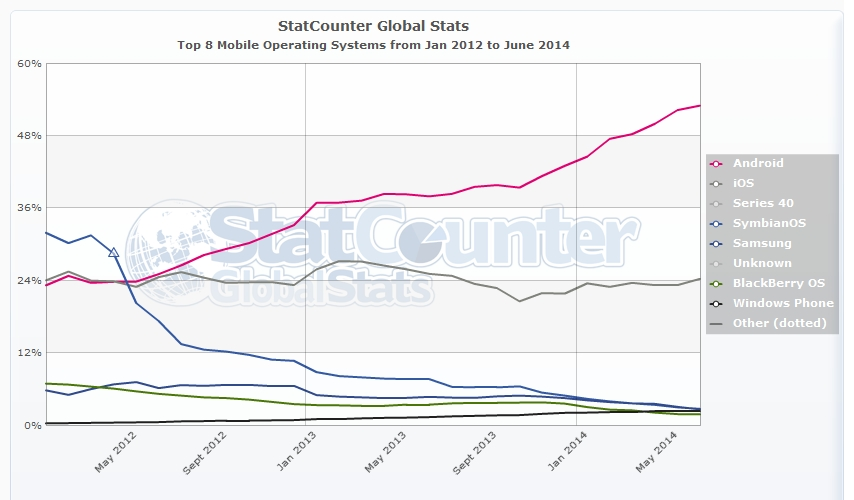
\includegraphics[scale=0.5]{Gambar/StatCounter} 
	\caption{Statistik Pengguna Windows Phone}
	\label{fig:StatCounter}
\end{figure}
\footnotetext[2]{\url{http://gs.statcounter.com/\#mobile_os-ww-monthly-201201-201406}} 

%Pragraf 4 latar belakang berisi ketertarikan penulis
\hspace{0.5cm} Berdasarkan hal tersebut, penulis mencoba mengembangakan aplikasi Pencarian Rute Kendaraan Umum di Windows Phone dalam tugas akhir ini. Aplikasi yang penulis kembangan akan memungkinkan pengguna menemukan rute kendaraan umum untuk sampai di tujuan. Untuk memudahkan pengguna, penulis akan menampilkan dalam 2 bentuk yaitu peta dan daftar. 

\section{Rumusan Masalah}
\label{sec:rumusan_masalah}
Sehubung dengan latar belakang diatas timbul permasalahan sebagai berikut:
\begin{itemize}
	\item Bagaimana membuat aplikasi di Windows Phone?
	\item Bagaimana mengintegrasikan Kiri API dengan aplikasi pencari rute kendaraan umum di Windows Phone?
\end{itemize}

\section{Tujuan}
\label{sec:tujuan}
Berdasarkan rumusan masalah pada sub bab 1.2, maka tujuan dari pembuatan tugas akhir ini adalah:
\begin{itemize}
	\item Mempelajari cara pembuatan perangkat linak di Windows Phone lalu mengembagan aplikasi yang akan dibuat.
	\item Membuat aplikasi di di Windows Phone yang memanfaatkan Kiri API.
\end{itemize}

\section{Batasan Masalah}
\label{sec:batasan_masalah}
Ruang lingkup pengembangan aplikasi Pencari Rute Kendaraan untuk Windows Phone ini dibatasi hal berikut:
\begin{itemize}
	\item Aplikasi ini akan berjalan di sistem operasi Windows Phone 8.
	\item Aplikasi ini membutuhkan koneksi internet.
	\item Aplikasi ini akan menampilkan rute jalur angkot, bus umum dan travel di tiga kota besar yaitu Bandung, Jakarta, dan Surabaya.  
\end{itemize}

\section{Metode Penelitian}
\label{sec:metode_penelitian}
Metode Penelitian yang penulis gunakan dalam membuat tugas akhir ini adalah sebagai berikut:
\begin{itemize}
	\item Melakukan studi pustaka mengenai XAML, kontrol dan navigasi di Windows Phone, Peta di Windows Phone, GPS di Windows Phone dan Kiri API.
	\item Melakukan analisis terhadap aplikasi lain yang menggunakan Kiri API.
	\item Melakukan analisis terhadap dasar teori untuk pembangunan aplikasi Pencarian Rute Kendaraan Umum untuk Windows Phone.
	\item Melakukan perancangan aplikasi Pencarian Rute Kendaraan Umum untuk Windows Phone.
	\item Implementasi dari aplikasi Pencarian Rute Kendaraan Umum untuk Windows Phone.
	\item Menguji aplikasi Pencarian Rute Kendaraan Umum untuk Windows Phone.
	\item Membuat kesimpulan.
\end{itemize}

%\section{Teknik Pengumpulan Data}
%\label{sec:teknik_pengumpulan_data}

\section{Sistematika Penulisan}
\label{sec:sistematika_penulisan}
%Bab 1
\hspace{0.5cm} Bab 1 membahas latar belakang masalah, rumusan masalah, tujuan penulisan tugas akhir, batasan masalah, ruang lingkup masalah, metode penelitian, dan teknik pengumpulan data tugas akhir ini.

%Bab 2
\hspace{0.5cm} Bab 2 membahas tentang teori-teori yang akan digunakan dalam tugas akhir ini. Bahasan yang dijelasakan pada bab ini adalah Windows Phone dan Kiri API. Teori Windows Phone yang dijelaskan meliputi lingkungan kerja, xaml, kontrol terhadap ponsel, siklus hidup aplikasi, peta di Windows Phone, lokasi, dan memanfaatkan sumber data. Teori Kiri API yang dijelaskan meliputi \textit{web service} penentuan rute, \textit{web service} pencarian lokasi, dan \textit{web service} menemukan transportasi terdekat. 

%Bab 3
\hspace{0.5cm} Bab 3 membahas tentang analisis pembangunan aplikasi Pencarian Rute Kendaraan Umum untuk Windows Phone. Pada Bab 3akan dibahas mengenai analisis kebutuhan aplikasi, analisis kontrol yang dipakai, analisis terhadap siklus hidup aplikasi, analisis terhadap siklus hidup aplikasi, analisis peta, analisis memanfaatkan sumber data, analisis Kiri API, diagram use case, dan diagram kelas.